%
% pathfinding implementation
% @author Tobias Weber <tweber@ill.fr>
% @date 2021
% @license see 'LICENSE' file
%

\chapter{Pathfinding Algorithm and Implementation}
\label{ch:impl}

In this chapter we describe the individual steps of the pathfinding strategy (see p. \pageref{sec:strategy})
in detail and at the same time present an implementation in C++ \cite{Stroustrup2008, Stroustrup2018}. 
Specifically, the latest version 20 of the C++ standard \cite{ISOCPP20} (C++20 in short)
was employed in the creation of the software, together with the Boost C++ template libraries \cite{web_boost}. 
The source code for the implementation can be found in the directory \lstinline|./src/core| 
together with the library routines in \lstinline|./src/libs| of the accompanying software.
Its Repository can be found at at \url{https://code.ill.fr/scientific-software/takin/paths}. 
Stable versions of the source code have furthermore been registered under the DOI 
\href{https://doi.org/10.5281/zenodo.4625649}{10.5281/zenodo.4625649}, please also refer to 
appendix \ref{ch:online} for more details.

Section \ref{sec:tasmodel} of the present chapter is dedicated to modelling the triple-axis spectrometer (TAS),
section \ref{sec:buildpath} discusses the steps involved in building up the mesh of possible instrument paths, 
and section \ref{sec:exepath} focuses on finding one specific path and executing the instrument motion along it.
The graphical and scripting user interfaces to the software are presented separately from the core functionality, 
namely in chapter \ref{ch:gui}.




% -----------------------------------------------------------------------------
% instrument model
% -----------------------------------------------------------------------------
\section{TAS instrument modelling}
\label{sec:tasmodel}
The very first task is to model the instrument space comprising the triple-axis spectrometer, the walls and
obstacles, as well as the floor as geometrical objects, for which positions and possible collisions can be
calculated. In the implementation, all these components are modelled hierarchically, starting at the top with the class
\lstinline[language=C++]|InstrumentSpace| which also serves as high-level interface for loading and saving
the instrument geometry and states. A domain model diagram of the class hierarchy can be seen
in Fig. \ref{ig:tas_class_hierarchy}.
State changes in the class, for example the occurrence of a collision, are signalled to the outside world
using the publish-subscribe mechanism via \textit{Boost.Signals2} \cite{web_boost_signals} library.
The publish-subscribe mechanism is also known as observer pattern, for which a comprehensive description 
can be found in Ref. \cite[Ch. 4, pp. 122-127]{FUH_prog2019}.

\begin{figure}
	\begin{center}
		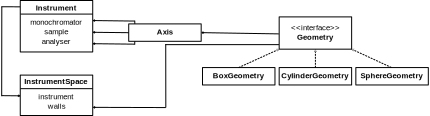
\includegraphics[width = 0.9 \textwidth]{figures/core_instrument_classes}
	\end{center}
	\caption[Instrument class hierarchy.]{Simplified domain model diagram of the triple-axis
		spectrometer. An instrument space consists of an instrument and a collection
		of walls. The instrument has three axes (monochromator, sample and analyser). The axes
		and the walls possess a specific geometry. The concrete geometries themselves implement
		the purely virtual class \lstinline[language=C++]|Geometry|.
		See Ref. \cite{web_domainmodeldiagram} for more information on these types of diagrams.
	\label{fig:tas_class_hierarchy}}
\end{figure}

The classes \lstinline[language=C++]|Instrument| and \lstinline[language=C++]|Axis| contain the actual
instrument definition. The spectrometer itself is also modelled as a hierarchy, namely of the
three principal instrument axes, among them the monochromator, sample and analyser.
In this respect it bears resemblance of a robot arm whose movement is restricted to a
two-dimensional plane.
Like in the modelling of a robot arm, each axis has three local coordinate systems, namely the
respective rotation relative to the incoming and outgoing vector, and an internal rotation which is
decoupled from the other local rotations.
Geometrical objects are derived from the abstract, purely virtual class \lstinline[language=C++]|Geometry|
and can be coupled to any of these three local coordinate systems.
This makes it possible to model neutron-optical components attached to either the incoming or
outgoing path of the neutron beam at the specific axis.
It furthermore enables us to have components which rotate independently of the axis,
for example a cryostat or a magnet on a separate rotation stage, as is usually the case in practice.
Physically, the outgoing angle of an axis is equal to the scattering angle of that axis, $2\theta_{M,S,A}$,
while the internal angles correspond to the respective crystal rocking angle, $\theta_{M,A}$ and $\Theta_{S}$,
where only the crystal is turned while keeping the scattering angle constant \cite[p. 87]{Shirane2002}
(see chapter \ref{ch:xtal}).
The transformation matrices corresponding to the three local coordinate systems are calculated as follows:
\begin{equation}
\begin{split}
	T_{\mathrm{in}}^{i} & \ =\  T_{\mathrm{out}}^{i-1} \cdot P^{i} \cdot R\left(\theta_{\mathrm{in}}^{i}\right), \\
	T_{\mathrm{int}}^{i} & \ =\  T_{\mathrm{in}}^{i} \cdot R\left(\theta_{\mathrm{int}}^{i}\right), \\
	T_{\mathrm{out}}^{i} & \ =\  T_{\mathrm{in}}^{i} \cdot R\left(\theta_{\mathrm{out}}^{i}\right).
\end{split}
\end{equation}
To facilitate rotation and translation in one step, the vectors and matrices for describing robot arms
are usually given in homogeneous coordinates \cite{Choset2010_ch3}, see also chapter \ref{ch:gl} for 
more mathematical details.

Here, the $T_{\mathrm{in,\, int,\, out}}^{i}$ name the transformation matrices of the incoming, internal (decoupled) 
and outgoing coordinate system of axis $i$, respectively.
$T_{out}^{i-1}$ is the outgoing transformation of the preceding instrument axis, or the identity if it is the first axis 
in the hierarchy.
$R\left(\theta_{\mathrm{in,\, int,\, out}}\right)$ are the corresponding rotation matrices and $P^i$ is the translation
of the local coordinate origin of the respective axis $i$.
The situation is depicted in Fig. \ref{fig:tas_axes}.


\begin{figure}
	\begin{minipage}{0.45 \textwidth}
		\begin{center}
			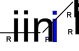
\includegraphics[width = 0.75 \textwidth]{figures/axis}
		\end{center}
	\end{minipage}
	%\hspace{1cm}
	\begin{minipage}{0.45 \textwidth}
		\begin{center}
			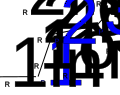
\includegraphics[width = 0.95 \textwidth]{figures/axes}
		\end{center}
	\end{minipage}
	\caption[Instrument axis coordinate systems.]{
	Left panel: Local transformations for an axis. The symbols $R_{\mathrm{x}}^i$ are shorthands
	for the rotation matrices $R\left( \theta_{\mathrm{x}}^i \right)$, with $x = \left\{ \mathrm{in,\, int,\, out} \right\}$.
	$P^i$ is the point of origin for the axis.
	Right panel: A hierarchy of three coupled axes build up the triple-axis spectrometer, with axes 1, 2, and 3 
	naming the monochromator, the sample, and the analyser axis, respectively.
	\label{fig:tas_axes}}
\end{figure}

% -----------------------------------------------------------------------------





% -----------------------------------------------------------------------------
% path building
% -----------------------------------------------------------------------------
\section{Construction of the path mesh}
\label{sec:buildpath}
This section is dedicated to calculating the path mesh, which consists of all possible instrument paths between
convex regions in configuration space. As seen in chapter \ref{sec:voro_median} and discussed in further detail
in section \ref{sec:polygonal_voronoi_diagram}, this mesh is to be equivalent to the 1-skeleton of the obstacle
boundary curves in configuration space.

As discussed in chapter \ref{sec:tasrobot}, path mesh creation will be based on the angular configuration space
(as opposed to -- for example -- crystal coordinates configuration space). 
The top-level C++ class for creating the path is named \lstinline[language=C++]|PathBuilder|. 
It mainly calls the low-level routines from the geometry library situated in the directory \lstinline|./src/libs| 
of the source code repository.


\subsection{Angular configuration space}
\label{sec:angular_config_space}
As the obstacles do not have any geometrically primitive shapes in angular configuration space, we need to quantise
the possible angular configurations into bins. We therefore iterate through the configuration space on a two-dimensional 
grid and create a bitmap of allowed and forbidden positions. The grid extends towards the scattering angles 
$2\theta_S \in \left[ -180^{\circ},\, 180^{\circ} \right]$ and monochromator angles of 
$2\theta_M \in \left[0^{\circ},\, 180^{\circ} \right]$, where, for the monochromator, we do
not use the full angular range as this is not possible in real instruments which have the monochromator at a 
fixed position and only scatter in one direction. The sample scattering angle, on the other hand, needs the full 
angular range as scattering on both sides of the axis is done in practice.

To check for the allowed positions, the instrument model, as is was described in section \ref{sec:tasmodel}, is
programmatically moved to each $\left( 2\theta_S,\, 2\theta_M \right)$ position on the grid and tested for
collisions with the walls or with itself.
Even though the instrument model itself is a three-dimensional representation of the spectrometer, we
can nevertheless simplify the collision detection checks to a two-dimensional plane. The reason for this is
that all possible obstacles in the instrument path, for instance walls and pillars, are upright and do not have
any sloped angles. And even if they were sloped, one can alternatively use the maximum extents, i.e. a bounding box,
in a two-dimensional representation and obtain the same results. The same is true for the instrument itself.
On the implementation side, the collision calculation on the two-dimensional grid is spread out on several
processor cores using the \lstinline[language=C++]|thread_pool| \cite{web_boost_asio_threadpool} class from the
\textit{Boost.Asio} \cite{web_boost_asio} asynchronous input/output library.
A thread pool maintains a fixed number of threads, $n$, onto which it loads a variable number
of tasks, $m$, where $m$ is usually larger than $n$. Each of the $n$ threads maintains a queue for the
threads it receives and processes them sequentially. A good explanation fo thread pools can be 
found in Ref. \cite[pp. 273-299]{Williams2012}.

With the given two-dimensional simplifications, we only need to distinguish three possible 
intersection tests for collisions: intersections between two polygons, which is done by an intersection
test between their line segments, line segment-circle intersections for the cases when a polygon 
collides with a circle, and circle-circle intersections. 
For efficiency, the actual calculations are only performed if the corresponding geometrical objects lie within 
one another's axis-aligned bounding boxes \cite{web_aabb}.

\subsubsection*{Line-line intersections}
We realised two different methods for checking if two line segments intersect.

\paragraph{Intersection check}
The first one is a check without calculation of the actual intersection point. 
This consists of testing if the two endpoints of line segment 1 are on two different sides of line
segment 2, and vice versa \cite{IntersectionCheck2021}. If both conditions are fulfilled, the two line segments intersect.
While this test is efficient in the number of calculations, we need to do $\mathcal{O}\left(n \cdot m\right)$ checks
to test the line segments of two polygons with $n$ and $m$ edges, respectively, for intersections with one another.

\paragraph{Intersection calculation}
For polygonal regions with a large number of edges, we implemented a sweep-based method which runs
in $\mathcal{O}\left(n \log n + k \log n\right)$ time for a total number of $n$ edges and $k$ points
of intersection between the lines \cite[p. 29]{Berg2008}.
It can be seen that while the individual calculations are more involved than in the simpler intersection check, 
they have to be performed less often for a large number of lines, $n$.

Before coming to the details, we first describe the calculation of the intersection of two lines in general.
Given two lines $\left|x_1\right> + \lambda_1 \left|d_1\right>$ and $\left|x_2\right> + \lambda_2 \left|d_2\right>$, 
the line-line intersection can be calculated by setting their equations equal, namely as follows \cite{wiki_line_line_intersection}:
\begin{equation}
	\left|x_1\right> + \lambda_1 \left|d_1\right> \ =\ \left|x_2\right> + \lambda_2 \left|d_2\right>,
\end{equation}
\begin{equation}
	\left|x_1\right> - \left|x_2\right> \ =\  \lambda_2 \left|d_2\right> - \lambda_1 \left|d_1\right>,
\end{equation}
\begin{equation}
	\left|x_1\right> - \left|x_2\right> \ =\  D \cdot \left| \lambda \right>,
	\label{eq:line_line_inters}
\end{equation}
where, in the last step, the matrix $D$ is composed of the direction vectors in its columns, $D = \left( d_2 \ |\  -d_1 \right)$, 
and the vector $\left| \lambda \right>$ has the two individual line parameter $\lambda_1$ and $\lambda_2$ in its
rows, $\left| \lambda \right> = \left( \lambda_2 \ |\  \lambda_1 \right)^T$.

For the given two-dimensional case, one can now directly solve for the $\lambda$s by left-multiplying with $D^{-1}$.
As the routine is also used by other code parts, we also include the general $n$-dimensional case in the implementation, 
determining the closest point between the two lines if no intersection exists.
This is done using the normal equation of the least-squares problem \cite[p. 793]{Arens2015}; 
the approximate version of Eq. \ref{eq:line_line_inters} thus reads \cite{wiki_line_line_intersection}: 
\begin{equation}
	D^T \left(\left|x_1\right> - \left|x_2\right>\right) \ =\  D^T D \cdot \left| \lambda \right>,
\end{equation}
\begin{equation}
	\left| \lambda \right> \ =\  \left( D^T D \right)^{-1} D^T \cdot \left( \left|x_1\right> - \left|x_2\right> \right).
\end{equation}

The intersection point (or the closest point) is thus found by inserting the $\lambda$ parameters in the respective line equation. 
Testing for the intersection of line segments instead of infinite lines is done by keeping the $\lambda$ parameters inside a given 
finite range.

For an efficient handling of multiple line segment intersections, the decision for which lines to test for intersections is
performed using the line segment sweep algorithm from Ref. \cite[pp. 69-80]{FUH_geo2020} whose C++ implementation can be
found in the function \lstinline[language=C++]|geo::intersect_sweep()| of the file \lstinline|./src/libs/lines.h| and which
is also described in the book by Berg \textit{et al.} \cite[Ch. 2, pp. 19-43]{Berg2008}.
We shortly summarise this algorithm and our implementation, following the description in \cite[pp. 69-80]{FUH_geo2020}:
\begin{enumerate}
	\item Possible events are kept in an event structure. Before the sweep, this is initialised with all the line segment
		endpoints. The structure itself is a priority queue which sorts its elements by their $x$ coordinate in ascending order.
		In the implementation we use the \lstinline[language=C++]|std::priority_queue| class of the C++ standard library.
	\item The line sweep is performed by iteratively taking the top element from the event structure's priority queue until
		the latter is empty, in which case the algorithm terminates.
		Depending on the type of the current element on top of the event structure, the following actions are performed:
		\begin{itemize}
			\item If the current event is the left endpoint of a line segment, the newly encountered line segment is
				inserted into the sweep status structure and is tested for intersections against its preceding and succeeding
				line segment in the status structure. Potential intersections are inserted into the event structure.
				The sweep status structure sorts the line segments according to their $y$ order at the current $x$ position
				of the sweep line. It is implemented using \textit{Boost.Intrusive}'s \cite{web_boost_intrusive}
				AVL tree class \cite{web_boost_intrusive_avltree} and can be found in the file \lstinline|./src/libs/trees.h|.
			\item If the current event is the right endpoint of a line segment, the now inactive line segment is
				removed from the sweep status structure and its preceding and succeeding line segments are tested
				for intersection. A potential intersection is inserted into the event structure.
			\item If the current event is an intersection point, the involved line segments are reported as intersecting
				and, as they cross at this point, their order is flipped in the event structure.
				After the flip, the intersecting line segments are tested against intersection with their new neighbours
				and the possible intersection points are inserted into the event structure.
				Note that in this method, we do need to calculate the actual intersection point, as it is at this point
				that we need to swap the order of the lines.
		\end{itemize}
	\item Repeat from step 2.
\end{enumerate}


\subsubsection*{Line-circle intersections}
As with the line-line intersection, we keep the problem general and directly look at the $n$-dimensional problem.
The intersection points between a line and an $n$-sphere are found by inserting the line equation 
$\left|p\right> = \left|x_1\right> + \lambda \left|d\right>$ into the sphere equation 
$\left< p-x_2 \ |\  p-x_2 \right> = r^2$, where $x_1$ names an arbitrary point on the line, $d$ its normalised 
direction vector, $x_2$ is the centre of the sphere/circle, and $r$ its radius \cite{wiki_line_sphere_intersection}.
The intersection points along the line are thus given by \cite{wiki_line_sphere_intersection}:
\begin{equation}
	\lambda \ =\ \left< x_2 - x_1 \  |\  d \right>
		\ \pm\ \sqrt{ \left< x_2 - x_1 \  |\  d \right>^2 
			+ r^2 - \left< x_2 - x_1 \ |\  x_2 - x_1 \right>}.
\end{equation}



\subsubsection*{Circle-circle intersections}
In this case we do not need the actual intersection points, so the calculation is restricted to checking if
the circles (or spheres) overlap. This is the case when the distance of their centres 
$\left| x_1 \right>$ and $\left| x_2 \right>$ is less than the sum of their radii, $r_1$ and $r_2$, respectively:
\begin{equation}
	\left< x_2 - x_1 \ |\ x_2 - x_1  \right> \ \leq \ \left( r_2 + r_1 \right)^2.
\end{equation}




\subsection{Representation of configuration space as spatial index tree}
\label{sec:walls_index_tree}
Having discretised the angular configuration space on a grid based on the intersections of the instrument
with the obstacle geometry or with itself, we next convert the positions
of all occupied bins on the grid, which represent these obstacles, in the form of a spatial index tree,
as described in chapter \ref{sec:indextrees}.
When calculating cost functions for different path finding strategies in one of the upcoming steps 
(section \ref{sec:optimalpath}), we can make use of the index tree for efficiently querying
the angular position of the wall that is closest to an arbitrary positions. 
It can furthermore be used to calculate the proximity of the instrument to the walls.

Internally, we make use of the R* tree implementation from Boost.Geometry's \cite{web_boost_geometry}
\lstinline[language=C++]|rtree| class \cite{web_boost_geometry_rtree}.
In our tests, the R* tree implementation proved far more performant than alternate tests using a k-d tree.
In the present use case, this is due to the fact that an R* tree is in smaller than the corresponding k-d tree
because vertices are grouped into tuples of, in our case, 8.



\subsection{Contour tracing}
\label{sec:contourtracing}
Having already determined a bitmap representation of allowed and forbidden regions in the angular configuration space,
we now need to trace the boundary contour between these regions.
To this end we use the radial sweep algorithm \cite{web_radial_sweep} whose implementation can be found
in the function \lstinline[language=C++]|geo::trace_boundary()| located in the file \lstinline|./src/libs/img.h|.

The radial sweep algorithm works as given below, following the descriptions in Ref. \cite{web_radial_sweep}:
\begin{enumerate}
	\item We scan the bitmap line by line and row by row until a forbidden region is found. 
		If the corresponding pixel has already been seen, we continue scanning. Otherwise it is marked as start pixel.
	\item We set an arbitrary direction vector pointing to one of the eight neighbouring pixels.
	\item The direction vector is rotated in a given, fixed sense, i.e. either in an always clockwise or 
		always counter-clockwise fashion, until the pixel it points to is again inside a forbidden region.
		If a full rotation has been performed without hitting a new forbidden region, the algorithm terminates.
	\item The current pixel position is incremented using the newly found direction vector. 
		We set the new direction vector to point from the new pixel to the old one and
		add the line connecting the old and the new pixel to the boundary.
	\item Step 3 is repeated until either the start pixel is seen again or no new direction vector is found.
\end{enumerate}



\subsection{Line segment generation and simplification}
\label{sec:line_seg_generation}
After the preceding step, we now possess a list of pixel coordinates marking the boundaries of occupied regions
in configuration space.
Panel (a) of Fig. \ref{fig:contour_simplification} shows a typical contour created by the angular sweep algorithm.
Line segments are now created between successive vertices, where one vertex is created for each pixel of the
quantified contour. The situation is shown in panel (b).

After creating the line segments from the traced contour lines, they have to be cleaned up and simplified,
because the quantity of superfluous vertices would considerably slow down the generation of the Voronoi 
diagram in a subsequent step of the path mesh building algorithm.
In the function \lstinline[language=C++]|geo::simplify_contour()|, which resides in the file \lstinline|./src/libs/hull.h|,
we perform two simplification steps:

First, ``staircase artefacts'' are removed. These kinds of artefacts originate from tracing diagonal or sloped lines.
The quantification of the obstacles on a grid and the subsequent run of the contour tracer (section \ref{sec:contourtracing})
create a succession of horizontal and vertical line segments in lieu of an actual diagonal.
The first simplification step, which is illustrated in panel (c) of Fig. \ref{fig:contour_simplification}, looks
for horizontal or vertical line segments between sloped line segments and removed the inner vertices and thus the
horizontal or vertical segments.

The second simplification step replaces collections of short collinear line segments with longer ones,
thus replacing the staircase artefacts, that the quantification step of the contour tracer had created,
with proper diagonal lines. This is depicted in panel (d) of Fig. \ref{fig:contour_simplification}.
To that end, we iterate through the vertices on the contour line and remove any vertices whose line segment angles
involving the previous and the next vertex, respectively, are below a given small scalar value $\epsilon$, with $\epsilon > 0$.


\begin{figure}
	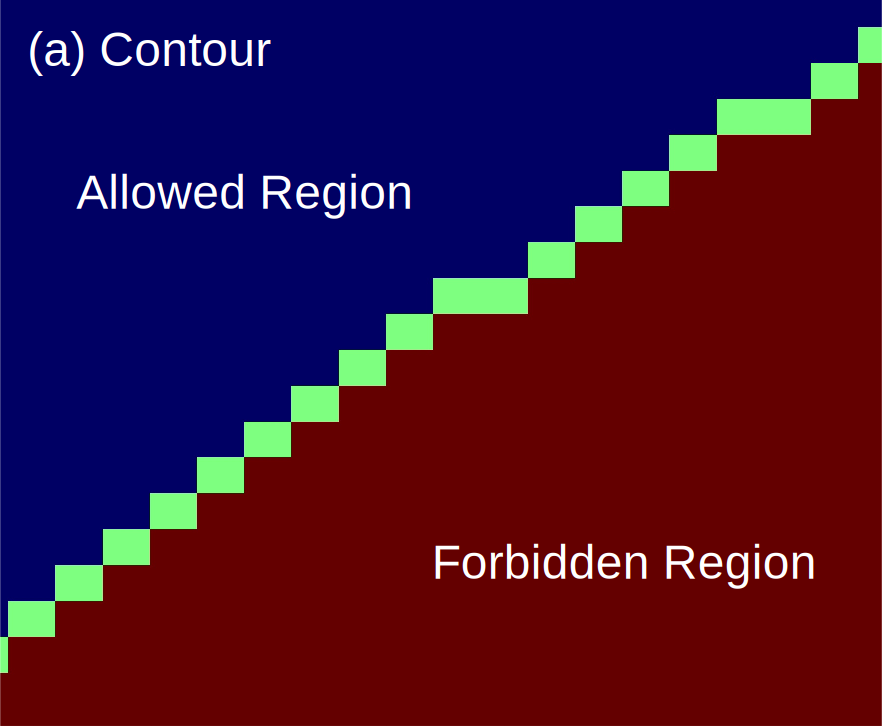
\includegraphics[width = 0.49 \textwidth, trim=0.25cm 0 0 0, clip]{figures/simplification_contour}
	\hspace{0.1cm}
	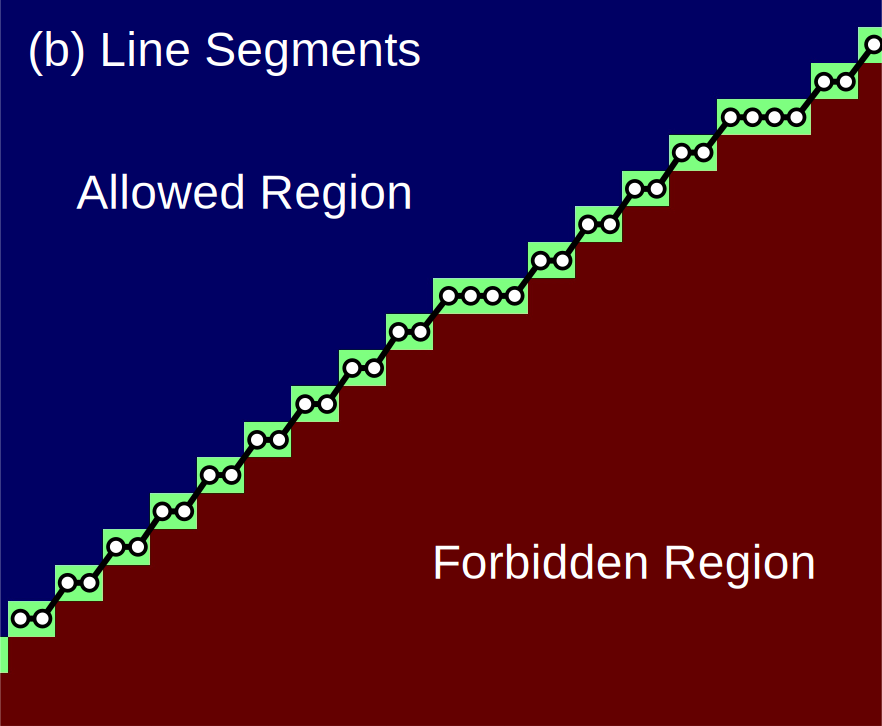
\includegraphics[width = 0.49 \textwidth, trim=0.25cm 0 0 0, clip]{figures/simplification_linesegments}

	\vspace{0.25cm}

	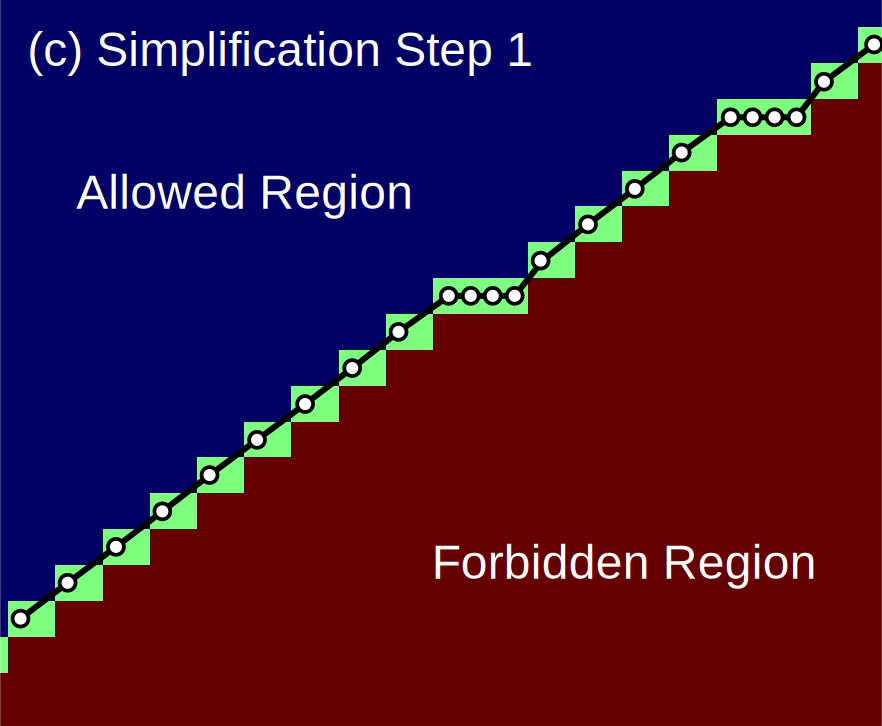
\includegraphics[width = 0.49 \textwidth, trim=0.25cm 0 0 0, clip]{figures/simplification_step1}
	\hspace{0.1cm}
	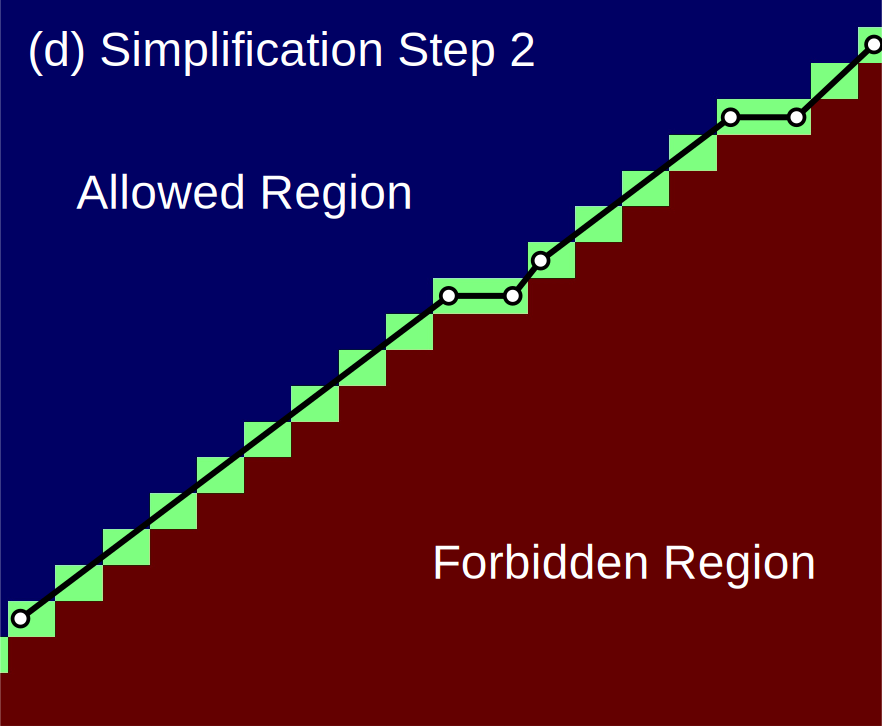
\includegraphics[width = 0.49 \textwidth, trim=0.25cm 0 0 0, clip]{figures/simplification_step2}
	\caption[Contour line segment generation.]{
		Typical example of a contour line segment generation and simplification.
		Panel (a): A contour line (green) separating two regions (blue and red) that have been found using 
			the tracing algorithm (section \ref{sec:contourtracing}).
		Panel (b): Vertices (while circles) are generated for each pixel and connected by line 
			segments (black lines).
		Panel (c): Staircase artefacts are removed from the line segment collection.
		Panel (d): Collinear line segments are merged and unnecessary vertices removed.
		\label{fig:contour_simplification}}
\end{figure}



\subsection{Generation of convex regions}
\label{sec:convex_regions}
The regions that were generated by contour tracing and line-segment generation in the previous steps are in general concave.
This can pose a problem, because we also need to be able to move the instrument into positions near concave angles
of the region's vertices, which generate ``alcoves'' in the region, see the next section for a discussion.

In this step, we thus split the regions into convex sub-regions. 
Note that in the final version of the code, this is implicitly handled in the next step, the generation of 
the Voronoi diagram. We nevertheless describe the idea and an explicit implementation.

The algorithm for splitting concave polygons into convex regions is given by D. Hegazy \cite{Hegazy2014},
on whose descriptions we base our present implementation.
The implementation can be found in the function \lstinline[language=C++]|geo::convex_split()| in the file
\lstinline|./src/libs/voronoi_lines.h| of our library .

The algorithm \cite{Hegazy2014} comprises four stages: 
\begin{enumerate}
	\item We iterate the vertices $v_i$ of the closed polygonal region and find concave corners.
		A corner is concave if the angle between three consecutive vertices is larger than 180 degrees,
		i.e. if $\angle\left(v_{i},\, v_{i+1},\, v_{i+2}\right) \, >\,  180^{\circ}$.
		If the polygon is already convex, that is, no such corner is found or the number of vertices is 
		equal or smaller than three, we stop.
	\item Having found a concave corner, we find the intersection of the edge line $l_i$, that is going 
		through the vertices $v_{i}$ and $v_{i+1}$, with the rest of the polygonal region.
		We remember the polygon vertex $v_j$ that follows on the contour after the intersection point $p$.
	\item We split the original polygon into two sub-polygons, with the vertices of sub-polygon 1 comprising
		$v_j,\, v_{j+1},\, ...,\, v_{i+1} $, and the vertices of sub-polygon 2 being $v_{i+1},\, v_{i+2},\, ...,\, v_j$.
		Alternatively, we could directly use the intersection point $p$ instead of the vertex $v_j$ for
		the split, but this would generate an additional vertex which was not in the original set.
	\item The algorithm is called recursively for the new sub-polygons 1 and 2.
\end{enumerate}
A visualisation and example run of the algorithm is shown in Fig. \ref{fig:contour_splitting}.


\begin{figure}[htb]
	\centering
	\includegraphics[width = 0.5 \textwidth]{figures/linesegs_convexsplit}
	\caption[Splitting of concave regions.]{
		Splitting a concave polygonal region into two convex sub-regions. The split is done 
		along the line segment $v_{i+1}$ $v_{j}$, where $v_j$ is the vertex next to the intersection
		point $p$ of the line $v_i$, $v_{i+1}$ containing the concave vertex $v_{i+1}$. See the text
		for details.
		\label{fig:contour_splitting}}
\end{figure}



\subsection{Calculation of the Voronoi diagram for polygons}
\label{sec:polygonal_voronoi_diagram}
As we are interested in the instrument path that is at the farthest position 
from walls, we need to calculate the Voronoi diagrams for the line segments 
that constitute these obstacles. 
In a second step, we group line segments into objects in to remove bisecting lines 
coming from the same object.
Please refer to chapter \ref{sec:voro} for a description of Voronoi diagrams, and
specifically to chapter \ref{sec:voro_ls} for line segment diagrams.

It is not sufficient to represent the walls as isolated line segments, because -- 
as we saw before -- they are not necessarily simply-connected. 
We rather represent them as concave or convex regions, of which we group all 
line segments that form the boundary of a simply-connected region.

The Voronoi diagrams only need to be calculated between such regions, 
the bisectors from line segments belonging to the same region are discarded. 
Fig. \ref{fig:linesegs_grouped_voro} shows an example of line segments and several
possibilities of grouping them. 
In case (a) they are not grouped and the Voronoi diagram is just the line 
segment Voronoi diagram. This case cannot be used for the paths of the spectrometer,
since the bisectors enter the forbidden region inside a wall.
In case (b) collections of line segments, which form arbitrary concave polygons, 
are grouped grouped into regions. Here, the bisectors do not touch any region 
and the resulting path is what is called the ``contour-parallel tool path'' in 
the terms of \textit{CNC} (computer numerical control) milling machines \cite{Jeong1998, wiki_milling}, 
a field where these kinds of paths are utilised. While the bisectors of this case could 
be used for the spectrometer path mesh, a problem remains: In contrast to a milling
machine the spectrometer is not supposed to be at the furthest distance of any
polygonal region at all times, but has a starting and ending position which can 
be close to one of these walls or be at a position near a concave corner which
is not directly accessible from the present bisector configuration. This problem
is solved in case (c).
In case (c) the concave polygonal regions are split into convex sub-regions, see
section \ref{sec:convex_regions}.
The bisectors form what is called a skeletal bisector configuration \cite{Jeong1998, Couprie2007},
and are closely related to the concept of the 1-skeleton or medial axis 
\cite[p. 111]{Boissonnat2006}, the generalised Voronoi diagram for curves that was 
discussed in chapter \ref{sec:voro_median}.
From the skeletal bisector mesh, each part of the instrumental configuration space 
can be reached, and no bisectors inside forbidden regions exit. 
This configuration will be used in the software for calculating the bisector 
path mesh for instrument movement.

In the implementation we distinguish between contours and inverted contours, with 
the former enclosing forbidden regions (and having an open allowed region outside) 
and the latter enclosing allowed regions (and having an open disallowed region outside).
This is a purely technical detail as mathematically the two cases are the same
with just the turning sense of the contour being different. 
Due to the nature of the contour-tracing algorithm (see section \ref{sec:contourtracing}), 
the turning sense of the contour is not preserved, and the nature of the contour 
and its regions have to be determined and stored separately.
Panel (c) of Fig. \ref{fig:linesegs_grouped_voro} shows the distinction: 
The contour of region 1 is an inverted one, as it encloses an allowed region,
whereas regions 2 and 3 are non-inverted, meaning they enclose forbidden regions.

Together with the calculation of the Voronoi diagram, a graph is constructed whose
vertices correspond to the Voronoi vertices of the diagram and whose edges correspond
to the Voronoi bisectors. 
Furthermore, a spatial index tree is created from the Voronoi vertices in the same 
step as the graph construction.
As before (section \ref{sec:walls_index_tree}), we again use the R* tree implementation
from Boost.Geometry's \cite{web_boost_geometry} \lstinline[language=C++]|rtree| 
class \cite{web_boost_geometry_rtree} (chapter \ref{sec:indextrees}).
The graph and the R* tree are queried in the pathfinding step described in
section \ref{sec:exepath}.

\paragraph{Implementation details}
The collection of normal and inverted regions is calculated in the member function
\lstinline[language=C++]|CalculateLineSegments()| of the \lstinline[language=C++]|PathsBuilder|
class, which resides in file \lstinline|./src/core/PathsBuilder.cpp|. 
The Voronoi diagram of these regions is calculated in the member function
\lstinline[language=C++]|PathsBuilder::CalculateVoronoi()|.
It calls the backend function \lstinline[language=C++]|geo::calc_voro()|, which is part
of the library and can be found in the file \lstinline|./src/libs/voronoi_lines.h|.

For the calculation of the line segment Voronoi diagrams the software uses either of two
backends, between which the user can freely switch: These are the the Voronoi 
extensions \cite{web_boost_polygon_voronoi} of the \textit{Boost.Polygon} 
\cite{web_boost_polygon, Simonson2009} C++ library for one,
and the \textit{2D Segment Delaunay Graphs} library \cite{web_2dsegdel, Karavelas2004, Karavelas2006} 
from the \textit{CGAL} software package \cite{web_cgal} for the other,
see the discussion in chapter \ref{sec:voro_ls}.

\begin{figure}
	\begin{minipage}{0.5 \textwidth}
		\begin{center}
			\includegraphics[width = 1 \textwidth]{figures/linesegs_ungrouped}
		\end{center}
	\end{minipage}
	\begin{minipage}{0.5 \textwidth}
		\begin{center}
			\includegraphics[width = 1 \textwidth]{figures/linesegs_grouped}
		\end{center}
	\end{minipage}
	\vspace{0.25cm}

	\begin{minipage}{0.5 \textwidth}
		\begin{center}
			\includegraphics[width = 1 \textwidth]{figures/linesegs_skeleton}
		\end{center}
	\end{minipage}
	\caption[Voronoi diagrams for polygonal regions.]{
		Panel (a): Ungrouped line segments and their Voronoi bisectors.
		Panel (b): The same line segments, but with each polygonal region grouped.
		The Voronoi diagram is only calculated between groups, not within the same group.
		Panel (c): A mixture of the first two cases, where not entire regions are grouped
		as in case (b), but where each convex sub-region forms its own group.
		\label{fig:linesegs_grouped_voro}}
\end{figure}

% -----------------------------------------------------------------------------





% -----------------------------------------------------------------------------
% instrument motion
% -----------------------------------------------------------------------------
\section{Finding the optimal path and the instrument motion}
\label{sec:exepath}

So far we have constructed a mesh of possible paths along which the instrument can 
potentially move from one convex region to another convex region of the angular configuration space.
In the present section we describe the algorithm to find a possible start position on the
path mesh to which the instrument can move from its initial configuration, which is
not necessarily on the path mesh (section \ref{sec:startend}).
Analogously, we determine the end position on the path mesh in proximity to the 
desired target instrument position.
A concrete path is then determined between the calculated start and end positions
(section \ref{sec:optimalpath}).


\subsection{Determination of the start and target coordinates}
\label{sec:startend}

For the start and target coordinate positions, which have their respective 
representation as large red and green points in Fig. \ref{fig:linesegs_path}, 
we find the closest points on the respective nearest Voronoi bisector and save 
these points as vertices on the generated path curve.
The closest Voronoi vertices to which these Voronoi edges belong are found by 
querying the R* tree that has been created in the mesh-building step of section
\ref{sec:polygonal_voronoi_diagram}.

In general, the closest point $\left|q\right>$ between a point $\left|p\right>$ 
and a line $l\left(\lambda\right) = \left|x\right> + \lambda \cdot \left|d\right>$ 
is determined by dropping a perpendicular from the point to the line \cite{wiki_proj}:
\begin{equation}
	\left|q\right> \ =\  \left<d  \ |\  p - x \right> \cdot \left|d\right>,
\end{equation}
where $\left|d\right>$ is the normalised direction vector of the line as depicted 
in Fig. \ref{fig:dropped_perpendicular}.
By reshuffling the equation, we can alternatively regard $\left|d\right> \left<d\right|$
as the operator projecting $\left| p - x \right>$ onto $\left|d\right>$, see \cite[p. 814]{Arens2015}.

\begin{figure}[htb]
	\begin{center}
		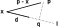
\includegraphics[width = 0.25 \textwidth]{figures/dropped_perpendicular}
	\end{center}
	\caption[Projection of a point onto a line.]{Projection of point $p$ onto line $l$.
		\label{fig:dropped_perpendicular}}
\end{figure}



\subsection{Calculation of the optimal path}
\label{sec:optimalpath}

Having found the points closest to the start and target positions on the bisectors, we can
proceed with calculating the optimal path on the path mesh formed by all Voronoi edges.
To this end, we make use of the graph representation of the Voronoi diagram that we calculated
in a previous step (section \ref{sec:polygonal_voronoi_diagram}) together with the diagram itself.
The graph's vertices and edges correspond to the Voronoi vertices and edges, respectively,
and the optimal path is determined using a cost function, which is applied to the graph's edge weights.

As discussed in chapter \ref{sec:dijkstra}, the optimal path minimising the edge weights 
can readily be calculated using Dijkstra's algorithm \cite{wiki_dijkstra}.
We now only need to specify a cost function to define what \textit{optimal} means exactly.

\paragraph{Shortest path}
The most obvious possibility for a cost function is the length of the Voronoi diagram's edges, 
for the linear bisectors this is simply the Euclidian 2-norm,
\begin{equation}
	f^{\mathrm{cost}}_1\left(\underline{v}, \underline{w} \right) \ = \ 
	\left\Vert \underline{v} - \underline{w} \right\Vert_2 \ =\ \sqrt{\sum_i \left(v_i - w_i\right)^2},
\end{equation}
where $v$ and $w$ name Voronoi vertices sharing an edge.
Using the edge lengths as as cost function leads to the path with the shortest distance 
between the start and target coordinates, i.e. the most basic application of Dijkstra's algorithm,
for which an example is shown in Fig. \ref{fig:linesegs_path}.

\begin{figure}[h]
	\begin{center}
		\includegraphics[width = 0.66 \textwidth]{figures/linesegs_path}
	\end{center}
	\caption[Path between a start and a target position.]{
		The final shortest path (orange) between the start and target positions (large red and green points, respectively).
		As before, the line segment vertices are depicted as blue points, the line segments as blue lines.
		The thin black lines represent the bisectors of the Voronoi diagram, the red points are the Voronoi vertices.
		\label{fig:linesegs_path}}
\end{figure}


\paragraph{Avoiding walls}
Berg \textit{et al.} mention a heuristic, non-analytic pathfinding approach using potential
functions \cite[p. 305]{Berg2008}. Their idea is to have the target position as a potential well attracting
the robot, and the walls and obstacles as repellant potential peaks. They, however, discuss
that such an approach can possibly trap the robot between several potential peaks.

For the present case, we can combine our analytical approach with the potential idea, but without 
resorting to heuristics. We can use the cost function to apply a potential, while keeping the
instrument position on the path mesh.
For the cost function, we keep the Euclidian distance between vertices, but include the vertices' 
distance from the closest wall in their vicinity as a repulsive potential. 
The simplest such potential is an $1/r$ function with $r$ being the closest distance from the 
Voronoi edge between two vertices to the next wall.
The cost function for two vertices $\underline{v}$ and $\underline{w}$ thus reads,
\begin{equation}
	f^{\mathrm{cost}}_2\left(\underline{v}, \underline{w} \right) \ = \ 
	\left\Vert \underline{v} - \underline{w} \right\Vert_2 \cdot \frac{1}{r}.
\end{equation}
The closest wall to an arbitrary point and thus the distance $r$ between them can be efficiently
determined using the spatial index tree that has been generated in a previous step
(section \ref{sec:walls_index_tree}).

A demonstration of the effect of the cost functions is depicted in Fig. \ref{fig:path_finding_strategies}.
More information on robot motion in potential function can be found in the notes by H. Choset \ref{Choset2010_ch4}.


\begin{figure}[h]
	\begin{center}
		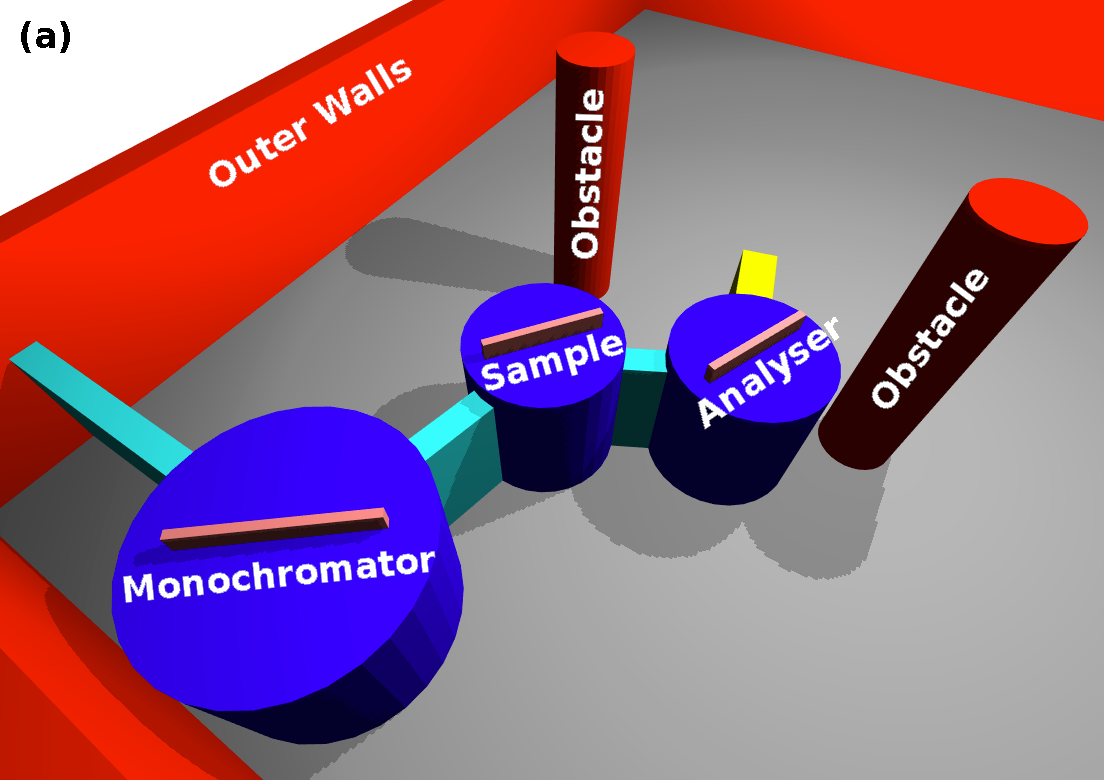
\includegraphics[width = 0.66 \textwidth]{figures/strategies_instrument}

		\vspace{0.1cm}
		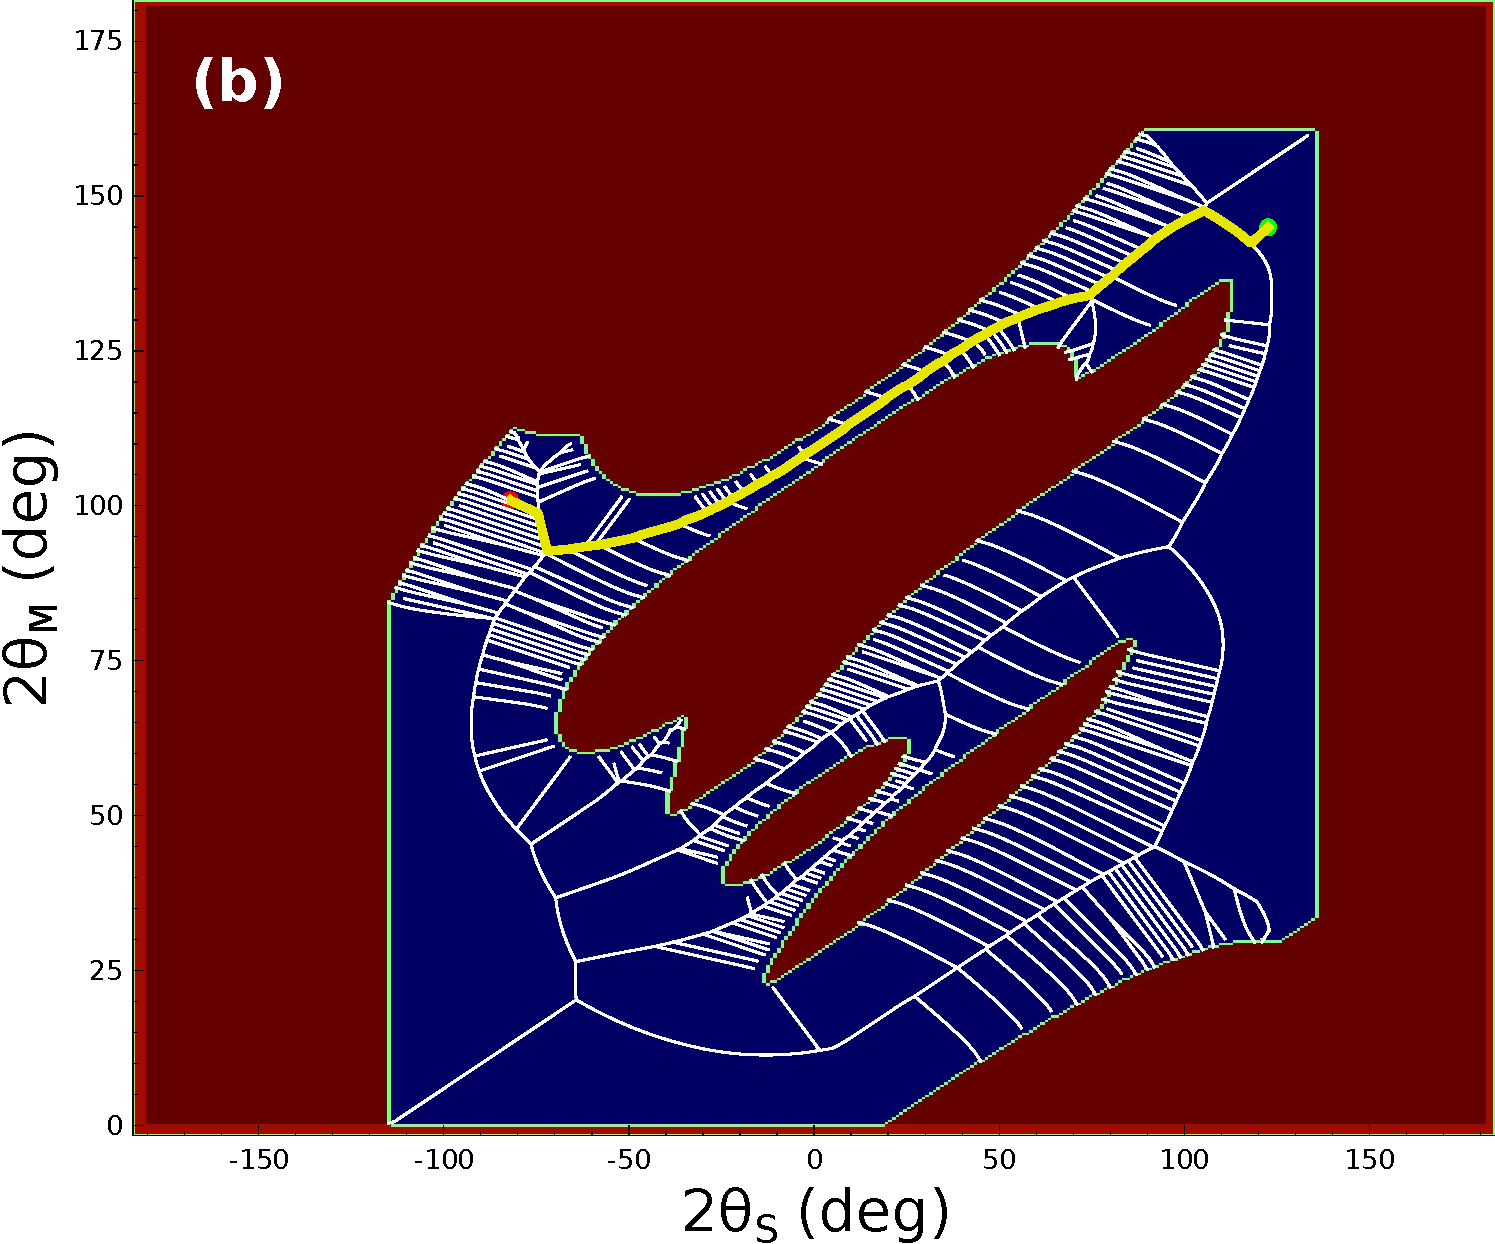
\includegraphics[width = 0.49 \textwidth]{figures/strategies_shortest_path}
		\hspace{0.1cm}
		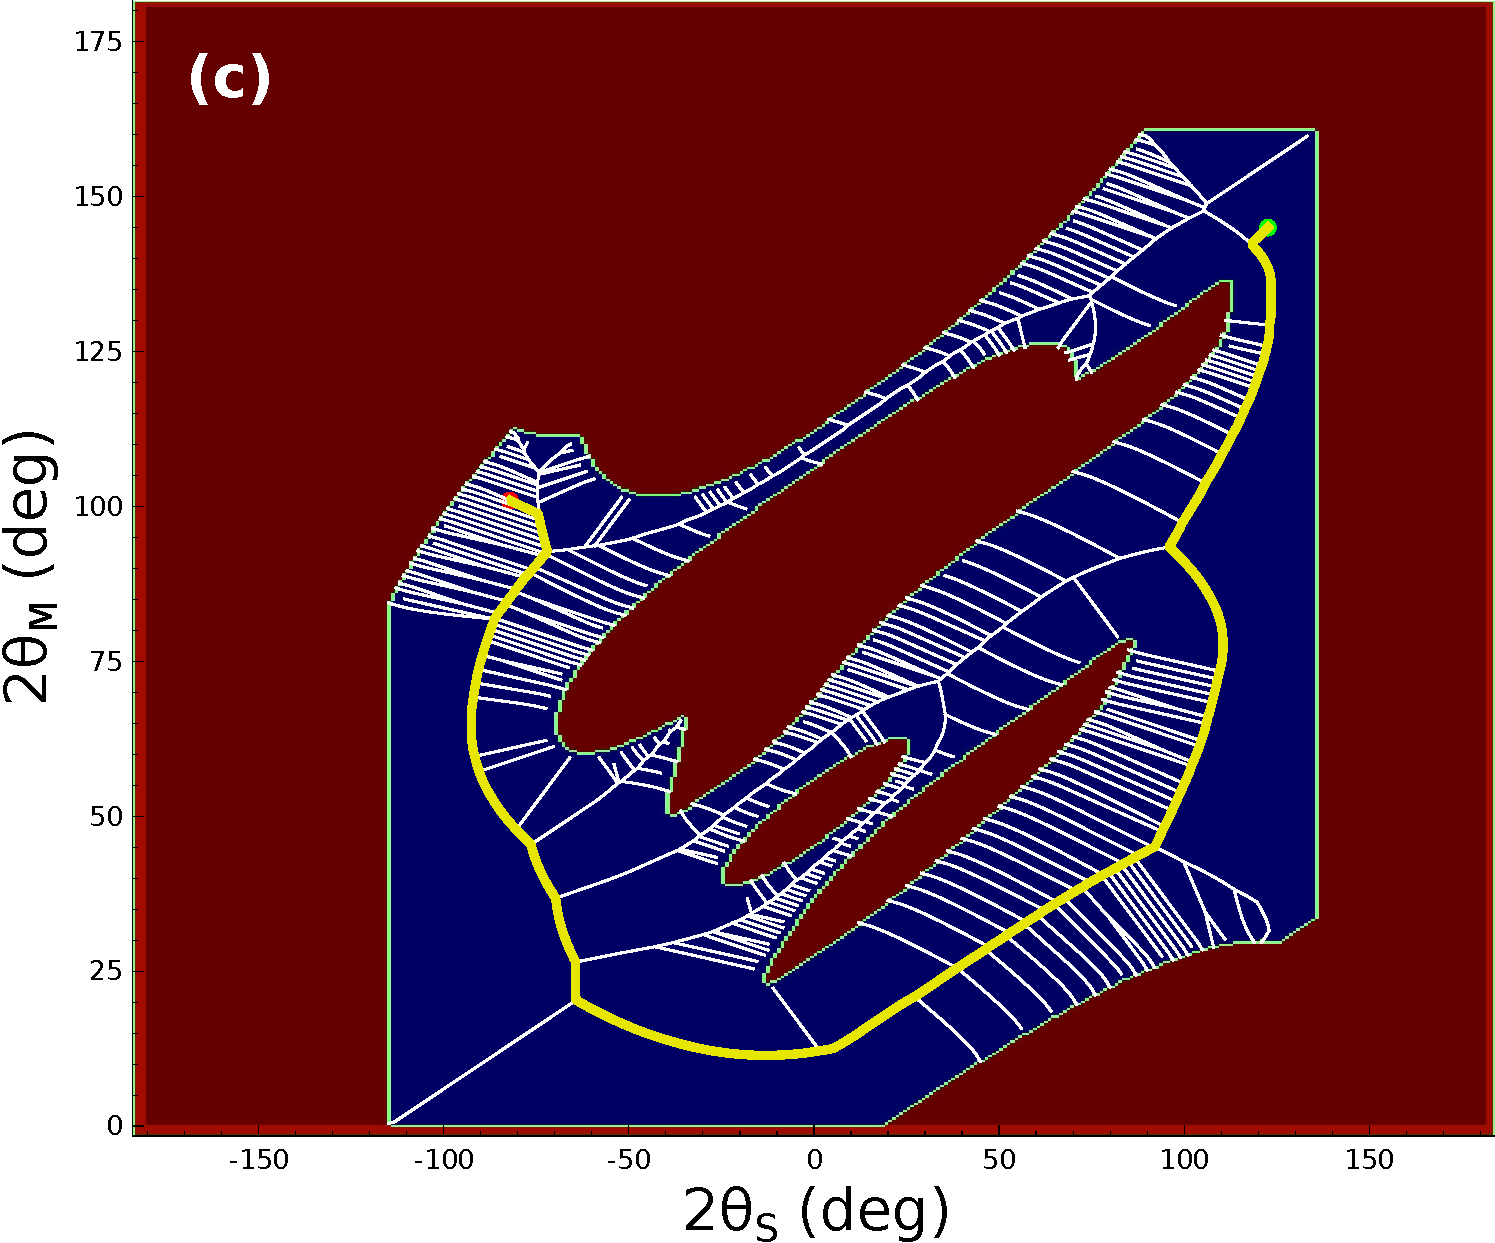
\includegraphics[width = 0.49 \textwidth]{figures/strategies_avoid_walls}
	\end{center}
	\caption[Pathfinding strategies.]{
		Effects of different cost functions on pathfinding.
		(a) The instrument is caught between two cylindrical obstacles.
		(b) The shortest path in angular configuration space moves the instrument very close to the obstacles.
		(c) The wall avoidance strategy chooses a longer, but safer path.
		\label{fig:path_finding_strategies}}
\end{figure}


\paragraph{Implementation details}
Our implementation of Dijkstra's algorithm, which can be found in the function 
\lstinline[language=C++]|geo::dijk()| of the file \lstinline|./src/libs/graphs.h|, is based on the 
pseudo-code given in Ref. \cite[p. 17]{FUH_algo_graphs_2021} together with the generalising modification of 
Ref. \cite[p. 285]{Erickson2019}. In the present implementation, the search for the next neighbour
to visit is performed using a heap data structure, whose construction and query is performed
using the standard C++ functions \lstinline[language=C++]|std::make_heap()| and 
\lstinline[language=C++]|std::pop_heap()|, respectively.
As it is compact enough and since it is representative of the design and coding styles of the software
in general, the implementation is printed in full in listing \ref{lst:dijkstra}.
Note that the implementation is generic, because it does not insist on a specific class
for the underlying graph. Instead it keeps the graph type, \lstinline[language=C++]|t_graph|, open and
only requires that it fulfill the template concept \cite{cppwiki_concepts}
\lstinline[language=C++]|is_graph|, which is given in listing \ref{lst:graph_concept}.
For the software package, we offer two graph implementations, one based on the adjacency list, the
other on the adjacency matrix, as discussed in chapter \ref{sec:graphs}.
The algorithm is furthermore agnostic towards the cost function and its interna and dependent 
data structures. To this end, a cost function can be provided as a generic callback function 
for which all the details are provided and only known by the caller.


\begin{listing}[htb]
	\begin{lstlisting} [language = C++,
			basicstyle = {\scriptsize},
			breaklines = true, tabsize = 4,
			numbers = left, numberstyle={\scriptsize}]
template<class t_graph,                           // generic graph and cost function types
	class t_cost_func = std::optional<typename t_graph::t_weight>(std::size_t, std::size_t)>
	requires is_graph<t_graph>                    // constrain graph type
std::vector<std::optional<std::size_t>>           // returns a vector of predecessors
dijk_mod(const t_graph& graph, const std::string& startvert,
         t_cost_func *cost_func = nullptr)        // optional cost function for edge weights
{
	// get start vertex index from its identifier
	auto _startidx = graph.GetVertexIndex(startvert);
	if(!_startidx) return {};                     // invalid identifier
	const std::size_t startidx = *_startidx;      // get the actual numeric start vertex index

	const std::size_t N = graph.GetNumVertices(); // number of vertices
	using t_weight = typename t_graph::t_weight;  // weight type from the generic graph type

	std::vector<t_weight> dists;                  // vectors of distances and predecessors
	std::vector<std::optional<std::size_t>> predecessors;
	dists.resize(N); predecessors.resize(N);      // allocate the space needed for N vertices

	// don't use the maximum, preventing overflows when we're adding the weight afterwards
	const t_weight infinity = std::numeric_limits<t_weight>::max() / 2;
	for(std::size_t vertidx=0; vertidx<N; ++vertidx)
		dists[vertidx] = (vertidx==startidx ? 0 : infinity);

	// comparator for distances, used for heap which implements the priority queue
	auto vert_cmp = [&dists](std::size_t idx1, std::size_t idx2) -> bool
	{
		return dists[idx1] >= dists[idx2];        // sort by ascending value: !operator<
	};

	std::vector<std::size_t> heap;                // heap with vertex indices,
	heap.reserve(N);                              // sorted by distances to start vertex
	heap.push_back(startidx);                     // only push start index, not all indices

	while(heap.size())                            // are there still elements in the heap?
	{
		std::size_t vertidx = *heap.begin();      // get the graph vertex on top of the heap
		std::pop_heap(heap.begin(), heap.end(), vert_cmp);
		heap.pop_back();                          // remove the top vertex from the heap

		// iterate the vertex' neighbours
		for(std::size_t neighbouridx : graph.GetNeighbours(vertidx))
		{
			// directly get edge weight, or use the user-supplied cost function
			std::optional<typename t_graph::t_weight> w = 
				cost_func ? (*cost_func)(vertidx, neighbouridx)
				          : graph.GetWeight(vertidx, neighbouridx);
			if(!w) continue;                      // ignore an invalid weight

			// is the path from startidx to neighbouridx over vertidx shorter
			// than from startidx to neighbouridx?
			if(dists[vertidx] + *w < dists[neighbouridx])
			{
				// update distances and predecessors
				dists[neighbouridx] = dists[vertidx] + *w;
				predecessors[neighbouridx] = vertidx;

				// insert the new vertex index if it's not in the queue yet
				if(std::find(heap.begin(), heap.end(), neighbouridx) == heap.end())
					heap.push_back(neighbouridx);

				// resort the priority queue heap after neighbouridx distance changes
				std::make_heap(heap.begin(), heap.end(), vert_cmp);
			}
		}
	}

	return predecessors;                          // return final vector of predecessors
}
	\end{lstlisting}
	\caption[C++ implementation of Dijkstra's algorithm.]{
	C++20 implementation of Dijkstra's algorithm, based on pseudo-codes from 
	Refs. \cite[p. 17]{FUH_algo_graphs_2021} and \cite[p. 285]{Erickson2019}.
	\label{lst:dijkstra}}
\end{listing}


\begin{listing}[htb]
	\begin{lstlisting}[language = C++,
			basicstyle = {\scriptsize},
			breaklines = true, tabsize = 4,
			numbers = left, numberstyle={\scriptsize}]
/**
 * requirements for the graph class interface
 */
template<class t_graph>
concept is_graph = requires(t_graph& graph, std::size_t vertidx)
{
	// function to get vertex count
	{ graph.GetNumVertices() }
		-> convertible_to<std::size_t>;

	// function to get vertex index from identifier
	{ graph.GetVertexIndex("v123") }
		-> convertible_to<std::optional<std::size_t>>;

	// function to get vertex identifier from index
	{ graph.GetVertexIdent(vertidx) }
		-> convertible_to<std::string>;

	// function to get edge weight
	{ graph.GetWeight(vertidx, vertidx) }
		-> convertible_to<std::optional<typename t_graph::t_weight>>;

	// function to get neighbours of a vertex
	graph.GetNeighbours(vertidx);

	// support insertion of vertices by identifier
	graph.AddVertex("v123");

	// support insertion of edges by index
	graph.AddEdge(0, 1);

	// support insertion of edges by vertex identifiers
	graph.AddEdge("v123", "v321");
};
	\end{lstlisting}
	\caption[C++ graph template concept.]{
	C++20 concept for a graph template class, \lstinline[language=C++]|t_graph|,
	constraining its interface to the one given here.
	\label{lst:graph_concept}}
\end{listing}



\section{Summary}
In summary, we presented a two-part pathfinding algorithm and its implementation, which generates an angular
representation of obstacles in a triple-axis instrument's path, calculates a mesh of skeletal bisectors between 
convex regions in its first part, and calculates an optimal path between user-specified start and target positions
in the second part. These positions can either be given as crystal coordinates or directly in angular configuration space.

The implementation of this algorithm so far is in the form of a C++ library. Several user interfaces, among them a
graphical one, have also been developed. These are described in chapter \ref{ch:gui}.
But before that, the upcoming chapter first describes some necessary basic concepts that are needed for the 
graphical representation of the data.

% -----------------------------------------------------------------------------
